\documentclass[11pt]{beamer}
\usetheme{Berkeley}

\usepackage[utf8]{inputenc}
\usepackage[T1]{fontenc}
\usepackage{amsmath}
\usepackage{amsfonts}
\usepackage{amssymb}
\usepackage{graphicx}
\usepackage{xeCJK}


\author{何静}

\title{生产与运作管理实务}

\logo{\includegraphics[width=0.1\textwidth]{../share/logo}}

\institute{东莞职业技术学院}

\date{2016年2月23日}

%\setbeamercovered{transparent}

\setlength{\parindent}{2em}
\setlength{\parskip}{0.5em}
\setlength{\baselineskip}{20pt}
\renewcommand{\baselinestretch}{1.25}

\begin{document}
	\maketitle
	
	\begin{frame}{目录}
		\tableofcontents
	\end{frame}
	
	\section{为什么要学习《生产与运作管理》}
	\begin{frame}{为什么要学习《生产与运作管理》}
		《生产与运作管理》是工商管理的专业核心课程。目的是使学生对生产运营管理的内容有全面的了解,掌握基本运作管理技术和方法,为将来进行生产或者服务管理打下良好的基础。
		
		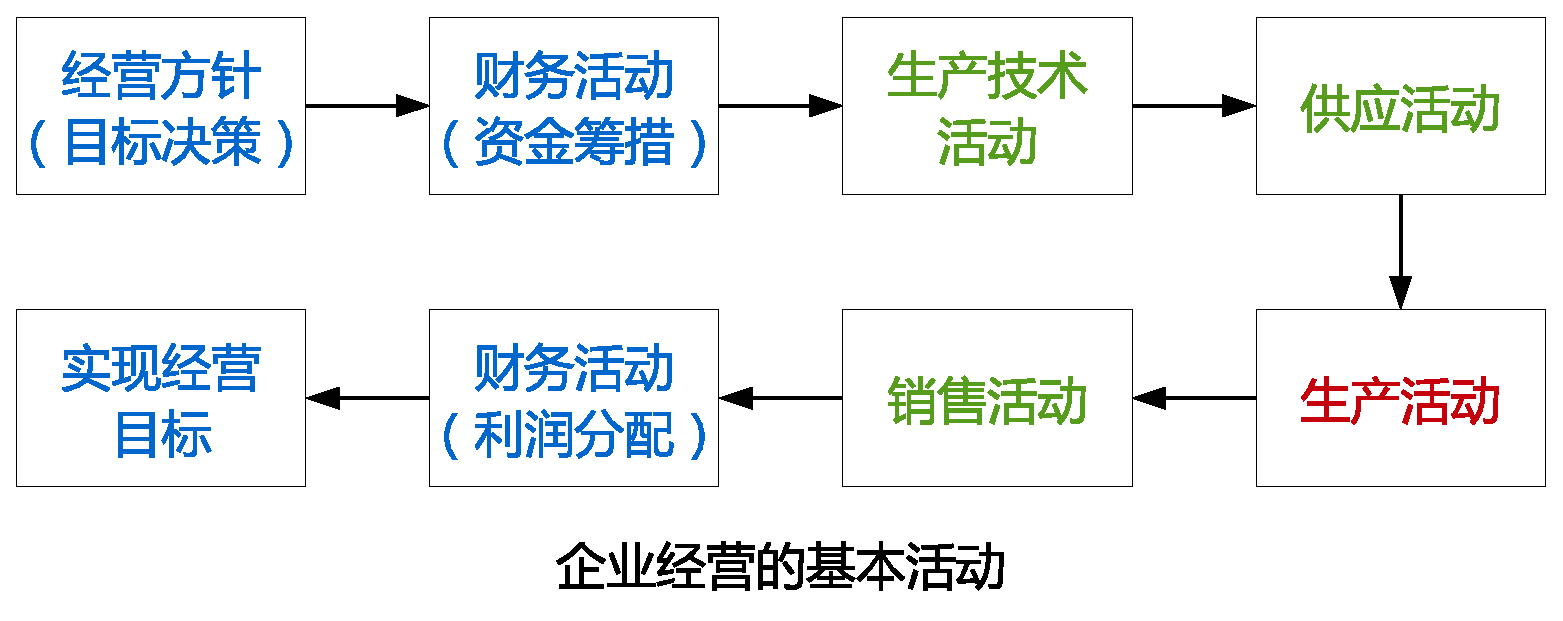
\includegraphics[width=0.9\textwidth]{img/生产活动}
	\end{frame}
	
	\section{“生产与运作管理”在企业中的地位}
	\begin{frame}{“生产与运作管理”在企业中的地位}
		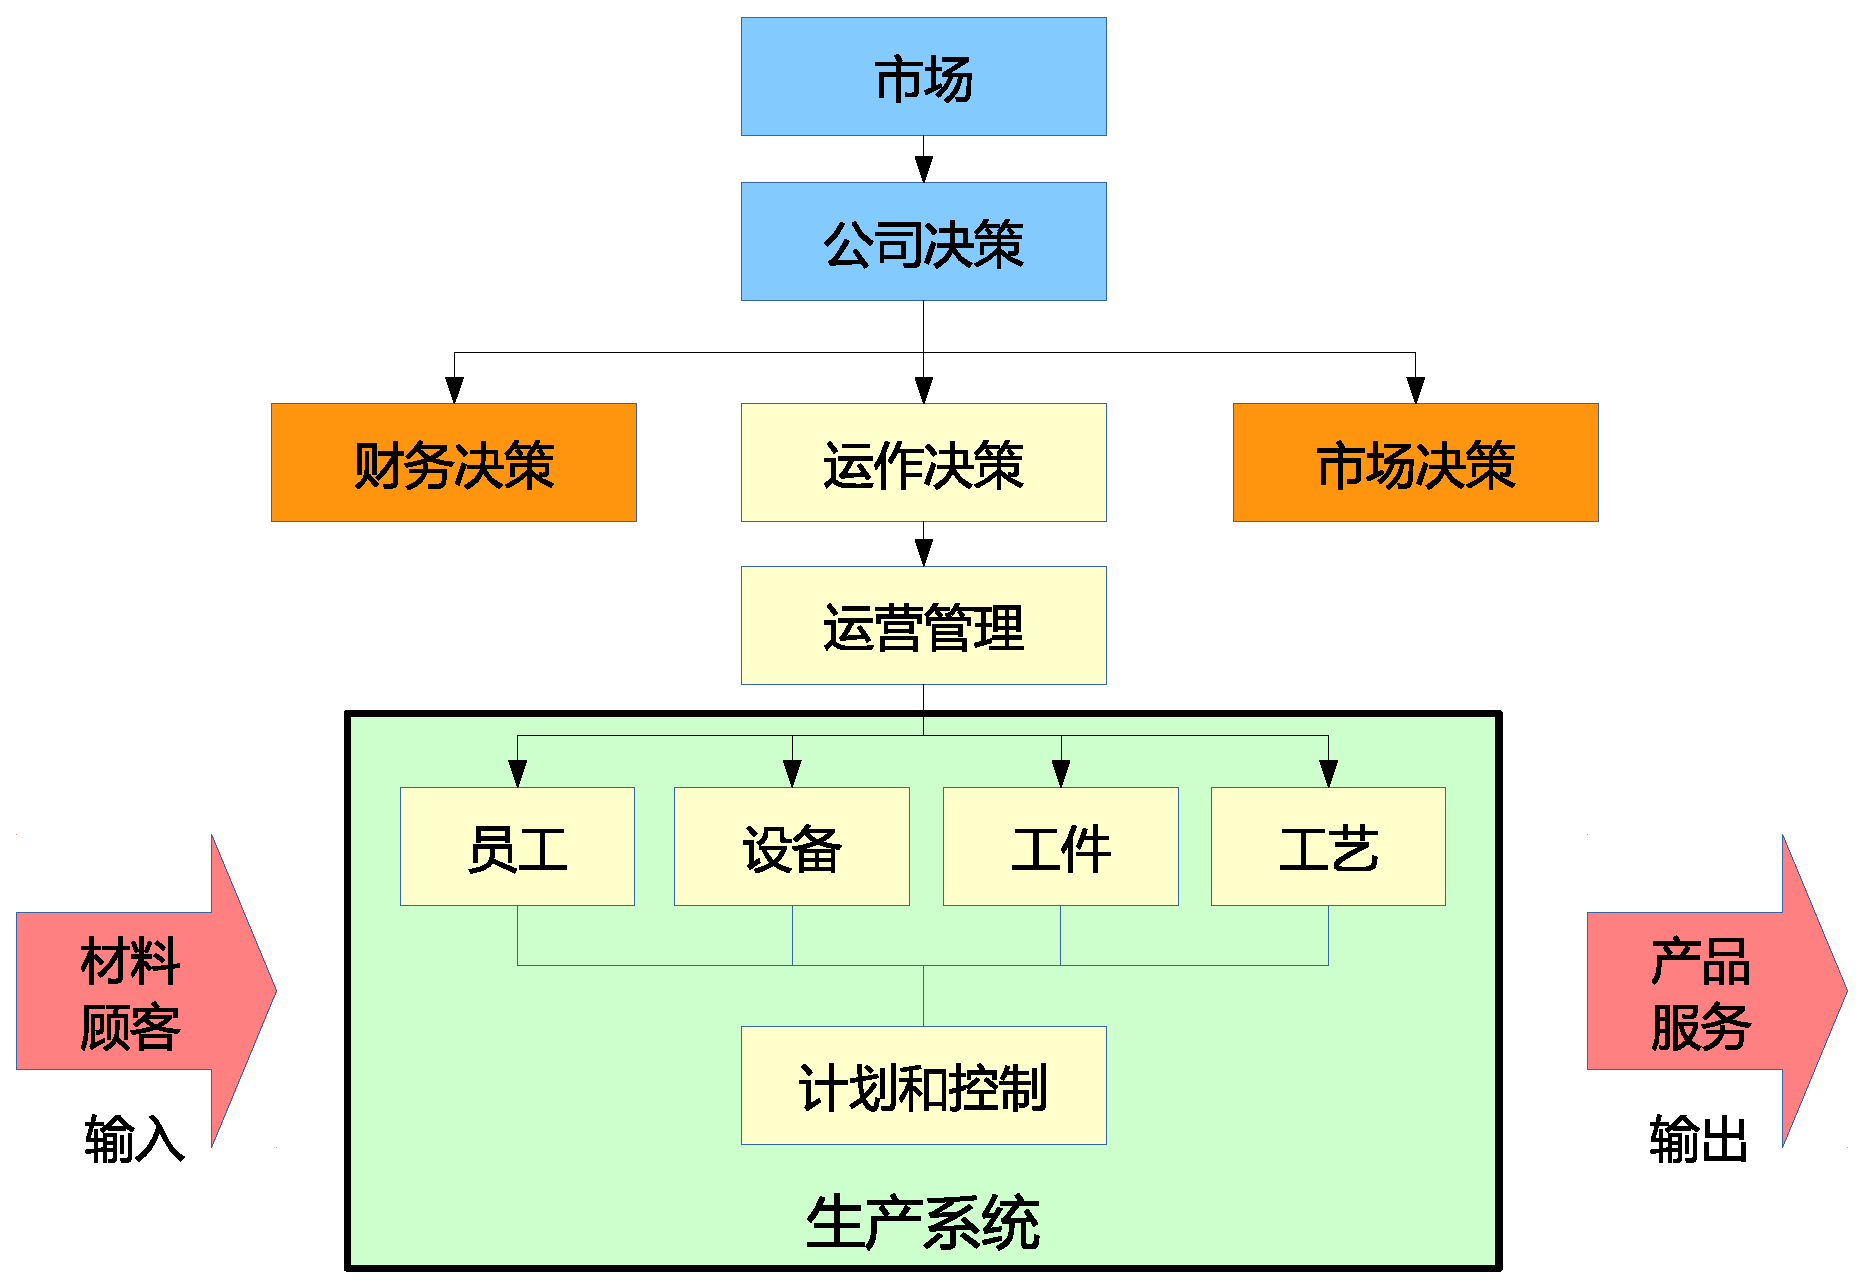
\includegraphics[width=0.9\textwidth]{img/生产系统}
	\end{frame}
	
	\begin{frame}{“生产与运作管理”在企业中的地位}
		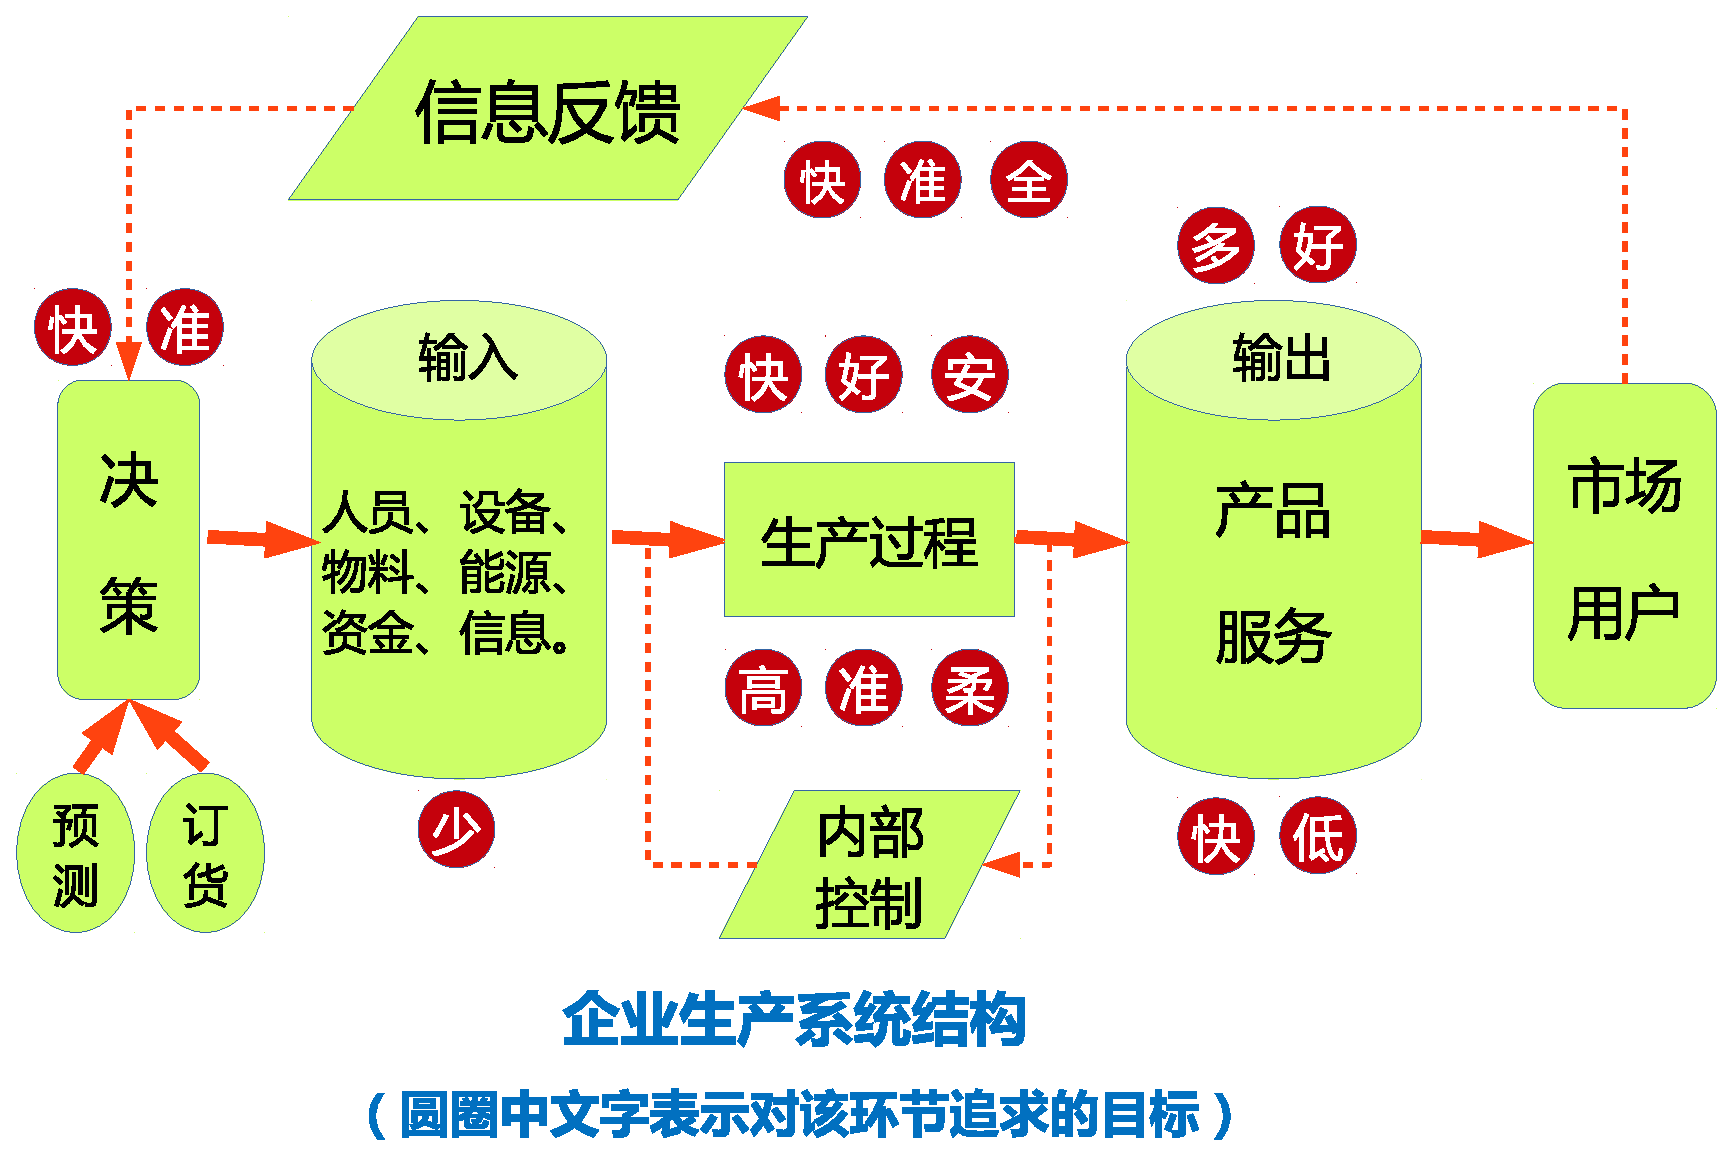
\includegraphics[width=0.9\textwidth]{img/生产系统结构}
	\end{frame}
	
	\section{为什么要学习《生产与运作管理》}
	\begin{frame}{为什么要学习《生产与运作管理》}
		\begin{block}{1、生产与运作管理是企业竞争力的源泉}
			企业的成败兴衰归根到底取决于它能否提供质量过硬、物美价廉、交货及时、服务优良的产品,特别是在市场变化多端、顾客需求越来越多样化的年代,生产与运作管理在企业全部经营管理活动中处于核心的地位。
		\end{block}		
	\end{frame}	
	
	\begin{frame}{为什么要学习《生产与运作管理》}
		\begin{block}{2、各类人员均须具备生产与运作知识(1)}
			\begin{itemize}
				\item 会计师需要了解库存管理、资源利用率和劳动定额才能够计算出精确的成本数据,从而进行审核,做出财务报告。
				\item 财务经理可运用库存和生产能力的概念来确定需要投入的资金量,预测现金流量,对现有资产进行管理。
				\item 营销专家需要了解怎样运作才能满足顾客定货日期,满足顾客对产品或服务的个性化要求以及进行新产品介绍。
			\end{itemize}  
		\end{block}		
	\end{frame}	
	
	\begin{frame}{为什么要学习《生产与运作管理》}
		\begin{block}{2、各类人员均须具备生产与运作知识(2)}
			\begin{itemize}
				\item 人事经理必须了解工作的设置、工作标准与员工激励方案之间的关系,以及生产工艺要求工人掌握的技术。
				\item 企业家往往因为没有良好的生产计划和库存管理的知识,不能有效地运用资金,而最终经营失败。
			\end{itemize}  
		\end{block}		
	\end{frame}
	
	\section{学习《生产与运作管理》的要求}
	\begin{frame}{学习《生产与运作管理》的要求}
		\begin{block}{《生产与运作管理》属于操作性很强的课程}
			\begin{itemize}
				\item 掌握《生产与运作管理》的基本概念、原理和功能。基本具备利用本课程知识分析和解决实际问题的能力。
				\item 掌握生产计划编制、质量管理、项目管理、库存控制等的基本概念、原理和方法。
				\item 了解现代生产和运作管理的发展趋势,掌握ERP系统的基本原理和方法。
			\end{itemize}  
		\end{block}		
	\end{frame}
		
	\begin{frame}{学习《生产与运作管理》的要求}
		\begin{block}{为什么不喜欢生产与运作管理}
			\begin{itemize}
				\item 对生产与运作管理的重要性认识不足。
				\item 生产与运作管理的复杂性。
				\item 枯燥。
			\end{itemize}  
		\end{block}	
		\pause
		\begin{block}{如何学“生产与运作管理”}
			\begin{itemize}
				\item 听明白。
				\item 注重图表和案例分析。
				\item 动手做。
			\end{itemize}  
		\end{block}	
	\end{frame}
	
	\section{《生产与运作管理实务》的内容和考试要求、}
	\begin{frame}{《生产与运作管理实务》的内容}
		\begin{itemize}
			\item 项目1  生产与运作管理概述
			\item 项目2  选址与设施布置
			\item 项目3  工作设计与组织
			\item 项目4  生产与运作计划
			\item 项目5  库存管理
			\item 项目6  MRP、MRPⅡ和ERP
			\item 项目7  质量管理与控制
			\item 项目8  生产现场管理与作业排序
			\item 项目9  项目管理和优化 
			\item 项目10  供应链管理
		\end{itemize}
	\end{frame}
	
	
	\begin{frame}{《生产与运作管理》的考试要求}
		\begin{block}{1.课堂教学:本课程共56学时(4*14)}
			\noindent 考核方式:(考试课)
			\begin{itemize}
				\item 考试成绩占60\%
				\item 平时成绩占40\%
			\end{itemize}			  
		\end{block}	
		\begin{block}{2.企业现场认知实训:1周}
			(具体见认知实习安排) 
		\end{block}	
	\end{frame}

\end{document}